%==============================================================================%
\section{Initial Experiments}
%==============================================================================%

With our theoretical understanding of the Wi-Fi standard and its capabilities, we move on to looking at the Wi-Fi landscape in real-world.
We achieve this by designing small independent experiments where we record the Wi-Fi probe requests within controlled conditions along with the knowledge of the ambient population of the field of measurement. 
We then look at the collected probe requests, examine them in detail to look at their properties, aggregate them to footfall counts and compare them with the real-world counts to get a overall idea of how well they translate into real counts.
The aim of these experiments to know more about the probe requests data and pick out the uncertainties and opportunities present in them.
The objectives here are,

\begin{enumerate}
  \setlength{\itemindent}{2em}
  \itemsep-0.25em
   \item Design a simple method to collect probe requests.
  \item Select locations with different levels of complexity.
  \item Collect real-world data through manual counting.
  \item Analyse the probe requests to extract useful information.
\end{enumerate}

%------------------------------------------------------------------------------%
\subsection{Experiment Design}
%------------------------------------------------------------------------------%

The first step was to design a simple method to collect Wi-Fi probe requests.
We accomplished this by using the open source, free software - \textit{tshark} \cite{wireshark2} on a regular laptop.
First we put the Wi-Fi module of the laptop in `Monitor mode' where it behaves as a wireless access point rather than a receiver.
Then we invoke the command line interface of the Wireshark programme - tshark to collect the Wi-Fi probe requests received by the laptop in Character Separated File (CSV) format. 
The full shell script which collects the data is given below,

\begin{minted}{bash}
#! /bin/bash
tshark \
  -I -i en0 \
  -T fields \
  -E separator=, \
  -E quote=d \
    -e frame.time \
    -e frame.len \
    -e wlan_radio.signal_dbm \
    -e wlan_radio.duration \
    -e wlan.sa_resolved \
    -e wlan.seq \
    -e wlan.tag.length \
    -e wlan.ssid \
  type mgt subtype probe-req and broadcast
\end{minted}

It is important to note that this script collects only particular data from the probe requests which we found to be relevant to us. 
The fields marked with \textit{-e} are the ones which were collected and the correspond to the information in the probe requests as follows,

\begin{enumerate}[rightmargin = 2em, leftmargin = 2em]
  \itemsep-0.25em
  \item \textit{frame.time} - Time stamp when the packet was received in microseconds.
  \item \textit{frame.len} - Total length of the packet in bytes.
  \item \textit{wlan\_radio.signal\_dbm} - Strength of the signal which delivered the probe request in dBm.
  \item \textit{wlan\_radio.duration} - The duration for which the signal has been transmitted.
  \item \textit{wlan.sa\_resolved} - The MAC address of the source device where the first part is resolved into a vendor name concatenated with 6 characters of the device part.
  \item \textit{wlan.seq} - Sequence number of the packet assigned by the source device.
  \item \textit{wlan.tag.length} - A list of lengths of the tags attached to the packet this acts a signature of the information contained within those tags and
  \item \textit{wlan.ssid} - The network for which the probe request is being sent for. This information is optional.
\end{enumerate}

The name of the manufacturer/ vendor of the Wi-Fi module  is extracted from the \textit{wlan.sa\_resolved} field into a separate column and the original field is hashed using the SHA256 algorithm implemented in R.
In addition to this, the pedestrians next to the sensor were counted manually by the surveyor.

%------------------------------------------------------------------------------%
\subsection{Living room}
%------------------------------------------------------------------------------%
The first set of experiment was conducted with the laptop in the researcher's living room.
The primary aim of this experiment to collect an initial set of probe requests to understand the information present in them in detail.
The living room had 2 Wi-Fi enabled device - an Android phone manufactured by Motorola and an Android TV box manufactured by Remix.
The house had 2 more phones - iPhone from Apple running iOS9 and an Android phone from Samsung in the rooms next door.
The script was left running in the laptop on 15 Nov 2015 from 19:44 to 21:15 with an unexpected failure of 15 minutes in between from 19:55 to 20:10 approximately.
In this duration, we collected around 3000 probe requests at the rate of 38 requests per minute.

\begin{marginfigure}
  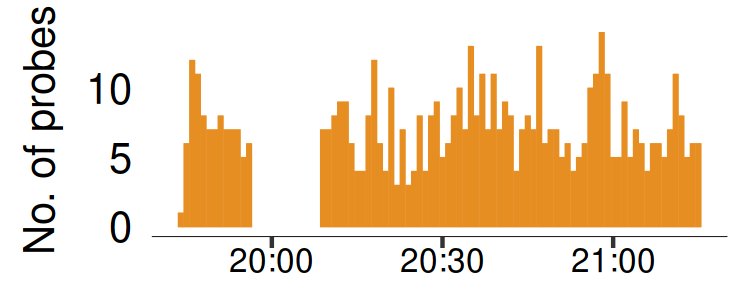
\includegraphics{images/home-total-count.png}
  \caption{Number of probe requests collected every minute on 15 October 2017}
  \label{figure:collection:home:total}
\end{marginfigure}

The first thing we tried with the probe requests is to try and aggregate them based on the MAC addresses.
Before the mobile devices started randomising their MAC addresses this should have accurately reflected the number of devices around the laptop.
The data when aggregated showed that there were around 211 unique MAC addresses recorded.
Being a residential area far away from traffic, these MACs are most likely not from unique devices.
The high number must be the result of randomisation.
More over since we know that there are only 2 - 4 devices in the house, there must be noise from significant distances beyond the house.
The number of unique MACs recorded every minute are shown in Figure \ref{figure:collection:home:total}
We observe that on average we captured around 7 unique MAC addresses every minute which quite far from the 2-4 range we were looking for.

Having established that just the MAC addresses are not enough to translate the probe requests into number of devices around the sensor, we started to look at other information we collected from the probe requests along with the MAC addresses.
First we tried to isolate all the randomised, local MAC addresses by looking at the resolved vendor part.
We aggregated the probe requests based on the vendor name present in the MAC addresses against all the other information present in them.
The results are shown in Table \ref{table:collection:proberequests}
We looked how many unique values were present in these fields compared to the total number of probe requests. 
Initially we assumed that the randomised one won't have OUIs which are public and hence the ones which can be resolved should be the real addresses.
But when we looked at the probes to MAC ratio of Google and Compex we realised that even the local MAC addresses could be registered public. 
This showed even when the OUI has been resolved into a vendor name, the original needs to be preserved for analysis.
Samsung is special case since we know from the specification that their devices do not randomise the addresses yet they have so many unique addresses which needs to be looked in to closely.

\begin{table}
\footnotesize
\begin{center}
  \begin{tabular}{lrrrrrrrr}
  \toprule
  Vendor & No. of & MAC & Signal & Frame & Dura-& Tags & SSID & Seq. \\ 
         & probes & addr. & (avg.) & length &  tion &  &  & no. \\ 
  \midrule
  AmazonTe &  101 &   1 & -80.53 &   4 &   4 &   5 &   3 & 101 \\ 
  Apple    &   77 &   7 & -86.29 &   4 &   4 &   9 &   4 &  77 \\ 
  ArrisGro &    7 &   1 & -91.71 &   1 &   1 &   1 &   1 &   7 \\ 
  Azurewav &  215 &   4 & -87.82 &   3 &   3 &  12 &  10 & 213 \\ 
  CompexPt &   75 &  28 & -88.17 &   3 &   3 &   5 &  29 &  74 \\ 
  CompexUs &    4 &   1 & -87.25 &   3 &   3 &   3 &   4 &   4 \\ 
  Dedicate &    2 &   1 & -92.50 &   1 &   1 &   1 &   1 &   2 \\ 
  Fn-LinkT &   64 &   1 & \textcolor{red}{-60.58} &   2 &   2 &   6 &   1 &  64 \\ 
  Google   & 1347 &  76 & \textcolor{red}{-69.14} &   4 &   5 &  41 &   6 & 1157 \\ 
  HuaweiTe &   11 &   3 & -87.91 &   3 &   3 &   3 &   1 &  11 \\ 
  IntelCor &   25 &   2 & -84.04 &   3 &   3 &   4 &   3 &  25 \\ 
  LenovoMo &    1 &   1 & -93.00 &   1 &   1 &   1 &   1 &   1 \\ 
  LgElectr &    1 &   1 & -90.00 &   1 &   1 &   1 &   1 &   1 \\ 
  Microsof &    3 &   1 & -90.00 &   1 &   1 &   1 &   2 &   3 \\ 
  Nvidia   &   65 &   1 & -82.91 &   2 &   2 &   4 &   2 &  65 \\ 
  OneplusT &    3 &   1 & -86.67 &   2 &   2 &   2 &   2 &   3 \\ 
  Pepwave  &    4 &   4 & -90.00 &   1 &   1 &   1 &   1 &   4 \\ 
  Sagemcom &    3 &   1 & -88.67 &   1 &   1 &   1 &   1 &   3 \\ 
  SamsungE &  655 &  27 & -83.81 &  26 &  26 &  54 &  23 & 621 \\ 
  SonyMobi &   56 &   2 & -78.66 &   2 &   2 &   2 &   1 &  56 \\ 
  TctMobil &    1 &   1 & -90.00 &   1 &   1 &   1 &   1 &   1 \\ 
  Tp-LinkT &   31 &   1 & -86.16 &   1 &   1 &   3 &   1 &  31 \\ 
  Wisol    &  143 &   3 & -71.91 &   4 &   5 &   6 &   3 & 142 \\ 
  XiaomiCo &    3 &   2 & -88.67 &   2 &   2 &   3 &   2 &   3 \\ 
  Unknown  &  110 &  40 & -88.86 &  19 &  18 &  21 &   5 &  90 \\ 
  \bottomrule
  \end{tabular}
\end{center}
\caption{Number of unique values present in each field captured from the probe requests aggregated by the vendor names}
\label{table:collection:proberequests}
\end{table}

We observe 24 different vendors in the data, even if we assume one device per vendor it is impossible for sensor to pick up 24 different devices without a significantly large area of measurement than we expect.
We need a way to filter out this noise which are generated from the edge of the field of measurement.
This is where the signal strength shows good promise.
Looking at the Table \ref{table:collection:proberequests} we can see that two of these vendors show significantly low average signal strength - Google and Fn-LinkT which can easily correspond to the two devices present in the room.
This can be explained by the decay of the signal as it passes through the walls.
In our simple example, we can filter almost all the noise with just the signal strength of the probe requests.

We then look at all the other information we collected from the probe requests and see how they compare to the MAC address for aggregating.
We observe that frame length and duration provides better aggregation into unique values than MAC address when they were randomised as seen with Compex and Google.
This can be explained by the argument that since the devices were essentially sending the same information over and over with just changed MAC addresses, which is are of fixed length, same devices should be sending packets of same length.
We also observe that duration of the transfer, being a function of the length of the signal, has almost the same amount of information in it as the frame length.
We can confidently pick one of these fields and discard the other for further analysis.
Though the tag lengths and SSID looked promising way to uniquely fingerprint the devices they don't have enough volume in them to offer substantial advantage.
The set of tag lengths are not as unique as the lengths or duration while the SSID information is sparse for most of the vendors.
For example, 66\% of probes with local OUIs, 50\% of the ones with Google and 38\% with Samsung don't have any SSID information in them.
This makes them very poor candidates for useful information in aid us with finger printing unique devices.

\begin{figure}
  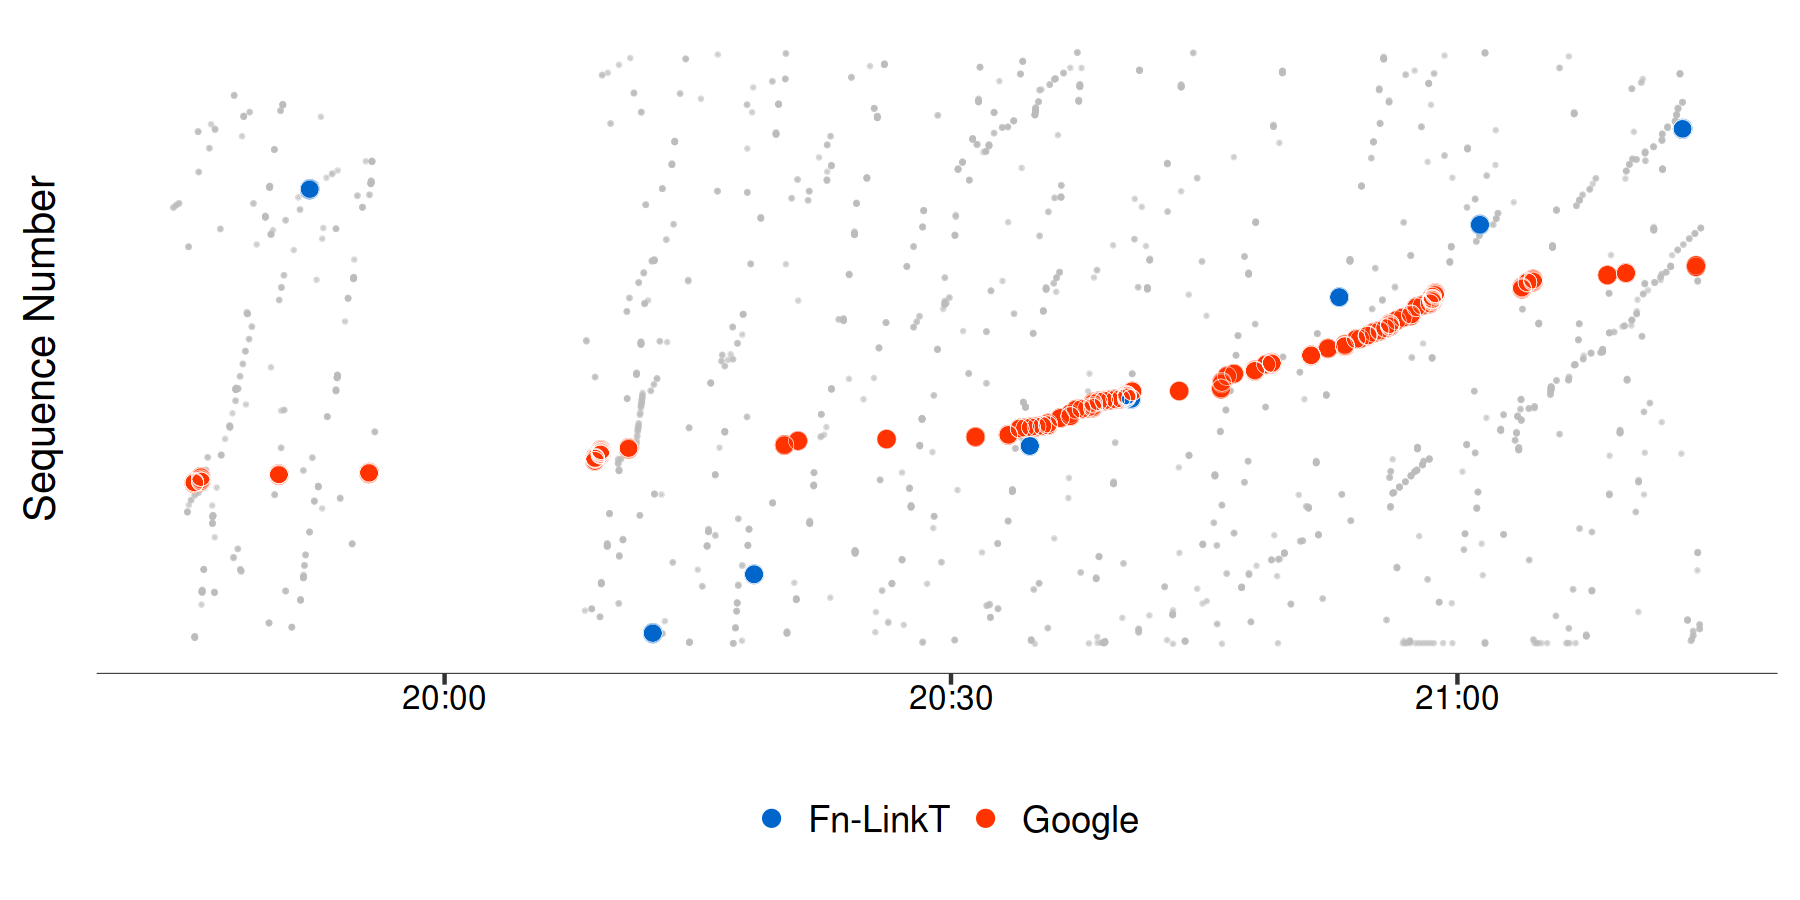
\includegraphics[trim = {0 10 0 0}, clip]{images/home-sequence-time.png}
  \caption{Sequence numbers plotted against timestamps showing clear patterns corresponding to unique devices.}
  \label{figure:collection:home:sequence}
\end{figure}
\marginnote{\textit{Grey dots are probe requests with signal strengths lower than -70dBm.} }

Finally we found that the sequence numbers are the most interesting part of the data collected. 
Though they don't uniquely identify the devices directly through aggregation, along with timestamps they form visually discernible, interesting patterns that correspond to the mobile devices that generated them.
In Figure \ref{figure:collection:home:sequence} we have isolated the two vendors - Fn\_LinkT and Google identified earlier and filtered only the probes requests with signal strength of more than -70dBm.
We then plotted their sequence numbers against the precise time stamps when they were received.
We can clearly see two devices which were present in the room and demonstrates the usefulness of sequence number in estimating the actual devices around the sensors.
We need to devise a method for isolating this `tracks' left by the devices in terms of their sequence numbers over time.
We can also observe the rotation of sequence numbers at 4096 for the Fn\_LinkT device which needs to be considered while devising such method.
Figure \ref{figure:collection:home:samsung} shows a similar exploration of Samsung devices.
Though from the table \ref{table:collection:proberequest} it looked as if Samsung devices are randomising their MAC addresses, we can clearly see in the figure that there are only two devices which were present for long time around the sensor and both did not randomise their addresses.
The diversity of MAC addresses were indeed unique devices which must be present far from the sensor.

\begin{marginfigure}
  \forcerectofloat
  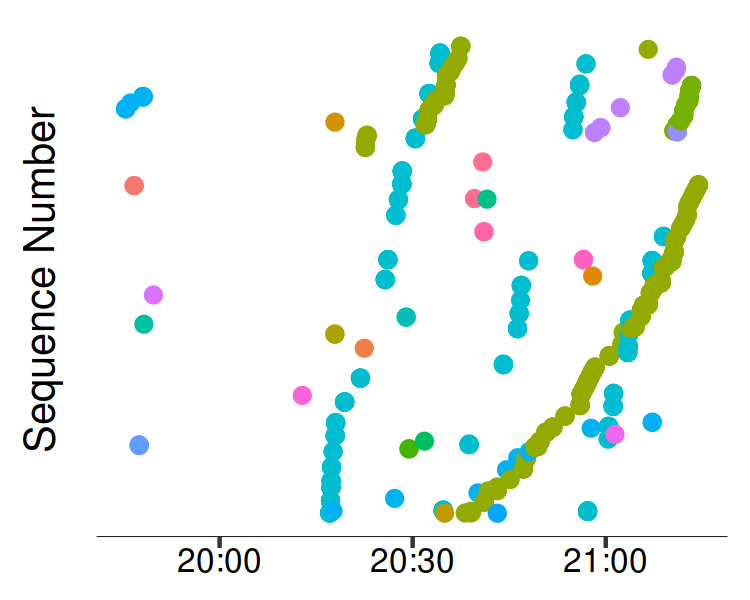
\includegraphics{images/home-samsung-google.png}
  \caption{Sequence number patters in Samsung devices showing the diversity of MAC addresses showing that they are not randomised.}
  \label{figure:collection:home:samsung}
\end{marginfigure}
\marginnote{\textit{The colours show unique MAC addresses.} }

To summarise, we found that even when an unique non randomised MAC address is present when collecting Wi-Fi probe requests, we get significant noise from outside the perceived field of measurement.
We also found that signal strength is a really good clue to filter out this noise.
The frame length and duration looks proimising for the same purposes but they utlimately have the same information and can be used interchangeable with similar results.
Finally we found that tag lengths and SSID are not useful information since they are either too varied or too sparse.
Though the results of this exploratory analysis has been positive the main challenge is to make sure these methods are feasible when dealing with more real-time, real world data.
We need to devise a more real world experiment to see frame lengths and signal strength work in a bigger data set for filtering out the noise. 

%------------------------------------------------------------------------------%
\subsection{UCL South Cloisters}
%------------------------------------------------------------------------------%

\begin{marginfigure}[4.5cm]
  \forcerectofloat
  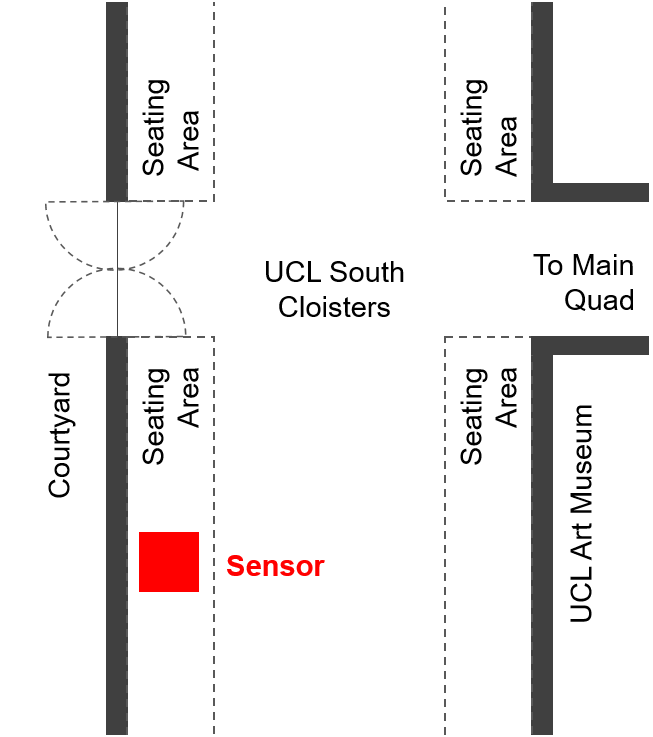
\includegraphics[trim={5 5 5 5},clip]{images/south-cloisters.png}
  \caption{Illustration showing the configuration of the sensor at UCL south cloisters}
  \label{figure:collection:ucl:config}
\end{marginfigure}
\marginnote{\textit{* Not to scale.} }

This experiment was conducted collect a broader dataset from a real world setting so that we can examine the results from the previous experiments with further confidence.
The specific goals were to validate the findings on signal strengths which correlated nicely to the distance from the sensor in the previous data and to further examine the usefulness of the frame length parameter.
We also wanted this to be a standard test dataset on which we can test our methodologies before they can be applied to a broader project such as Smart Street Sensors.
The data collection was conducted at one of the corridors in UCL - Southern cloisters which attracts a lot of pedestrian traffic during term time.
This corridor also has substantial seating areas along the sides where students usually sit down for long periods of time to work.
This provides us a source of devices which dwell near the sensors while constantly sending out probe requests.
This area is also used heavily for lunch and for exhibitions/ events attracting  large of visitors as well making it ideal for `stress testing' our methods for cleaning and aggregation.
The position of the sensor with respect to building is shown in \ref{figure:collecton:ucl:config}.
The data was collected from 15:37 to 16:20 on 04 December 2017 and in that duration we collected around 14,750 probe requests using the scripts mentioned earlier and we counted 652 pedestrians walking directly in front of the sensors manually with pen and paper.

Unlike the previously collected data in this experiment we made sure that the OUI information is preserved even after resolving them to vendor names.
With this information we looked at the second character of the OUI and categorised the probe requests as either 'local' - randomised or 'global' - non randomised.
We then compared them to the vendor names to find if any manufacturers other than google have registered OUIs in the local range.
Figure \ref{figure:collection:ucl;treemap} shows the distribution of vendors within both local and global range of OUIs in terms of the number of probe requests collected.

\begin{figure}
  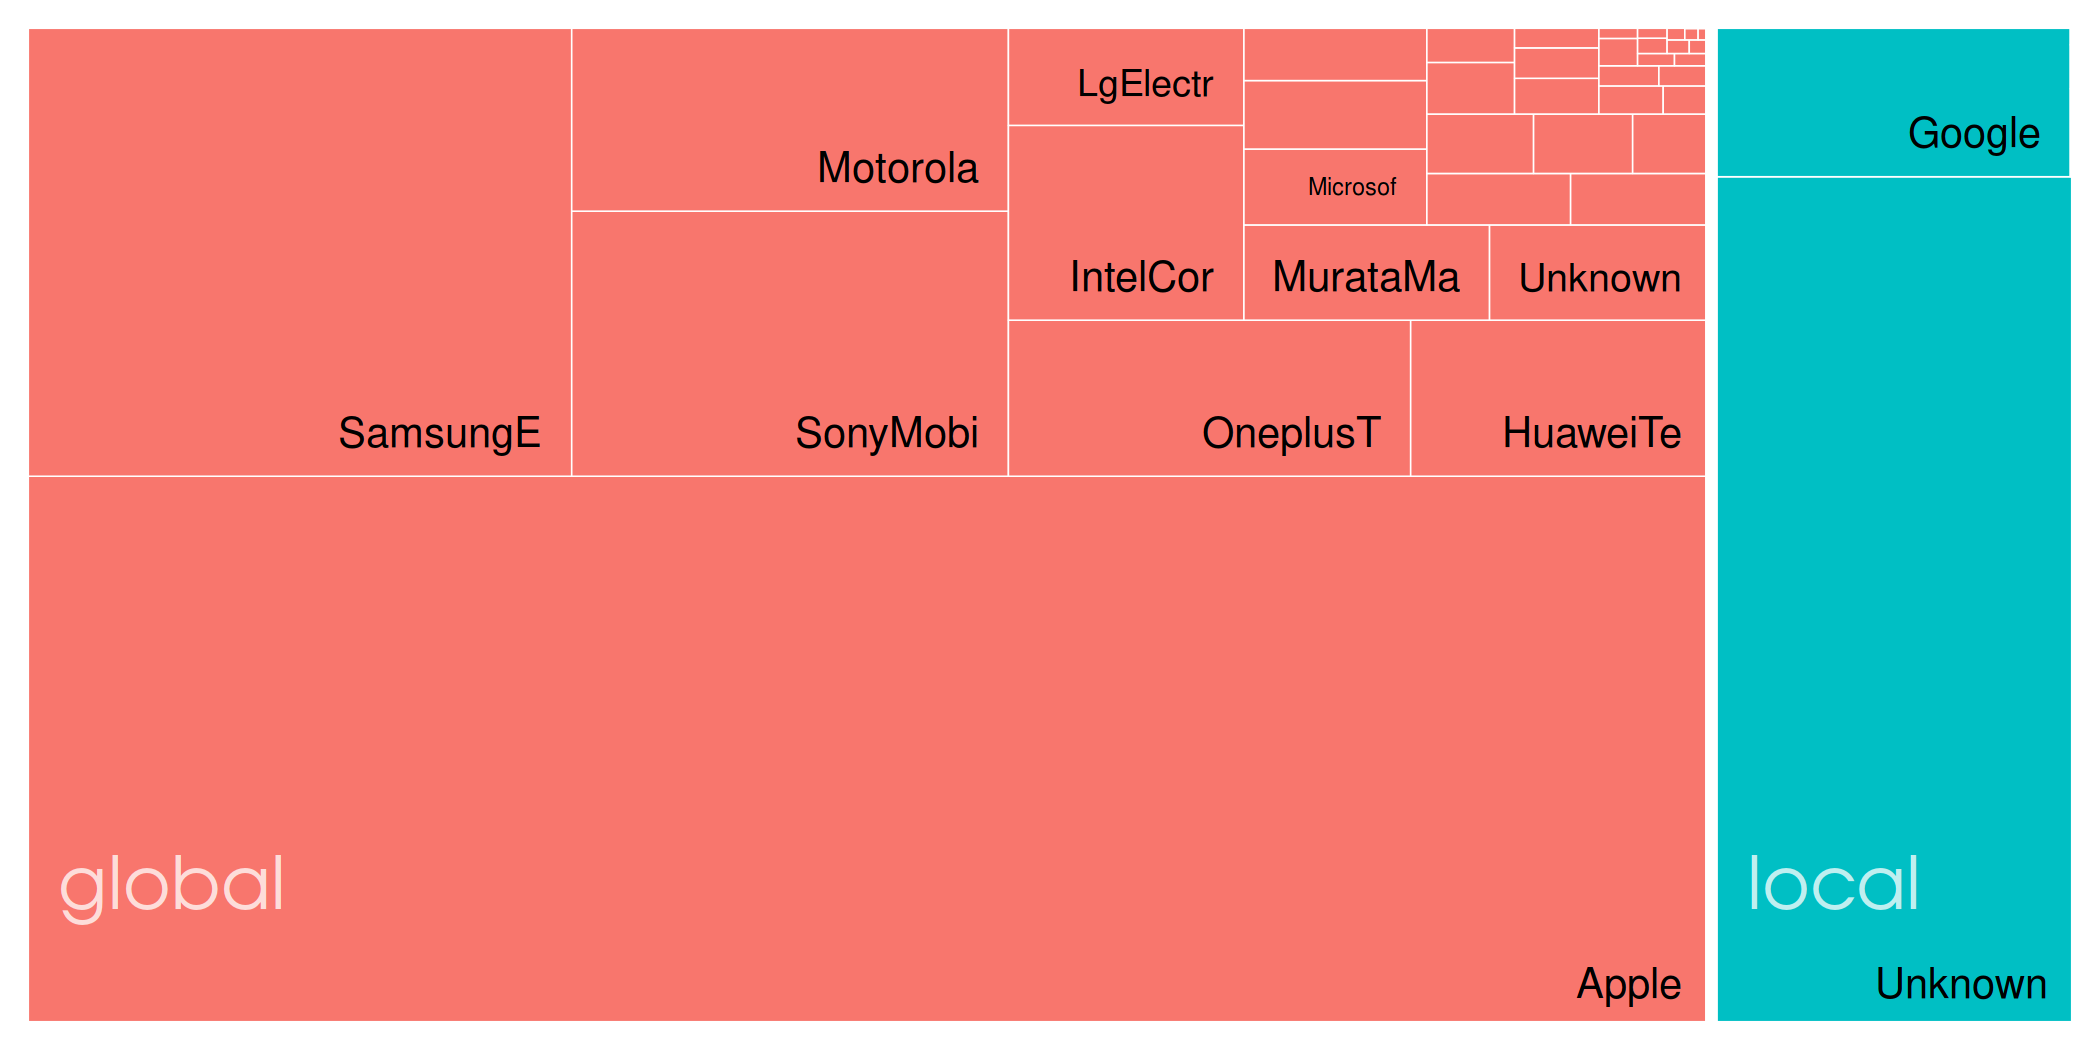
\includegraphics{images/ucl-local-treemap.png}
  \caption{Number of probe requests collected every minute on 15 October 2017}
  \label{figure:collection:ucl:treemap}
\end{figure}

We observe that Google is the only registered public OUI we find in the public range. 
We also noticed that the percentage of global MAC addresses collected was unusually large - 82\%.
This can be explained by the behaviour of the Apple devices while randomising the MAC addresses. 
Apple phones are known to randomise their addresses while probing for access points only when they are not connected to a Wi-Fi network already as documented by \citet{vanhoef2016}.
Since most of the members of UCL have access to `eduroam' network and are connected to it at the campus, most of the apple devices we captured haven't randomised their addresses.
This made this dataset heavily biased and not suitable for testing device finger printing methods but it does give us an opportunity to examine the nature of probe requests generated by Apple devices in particular.

\begin{figure*}
  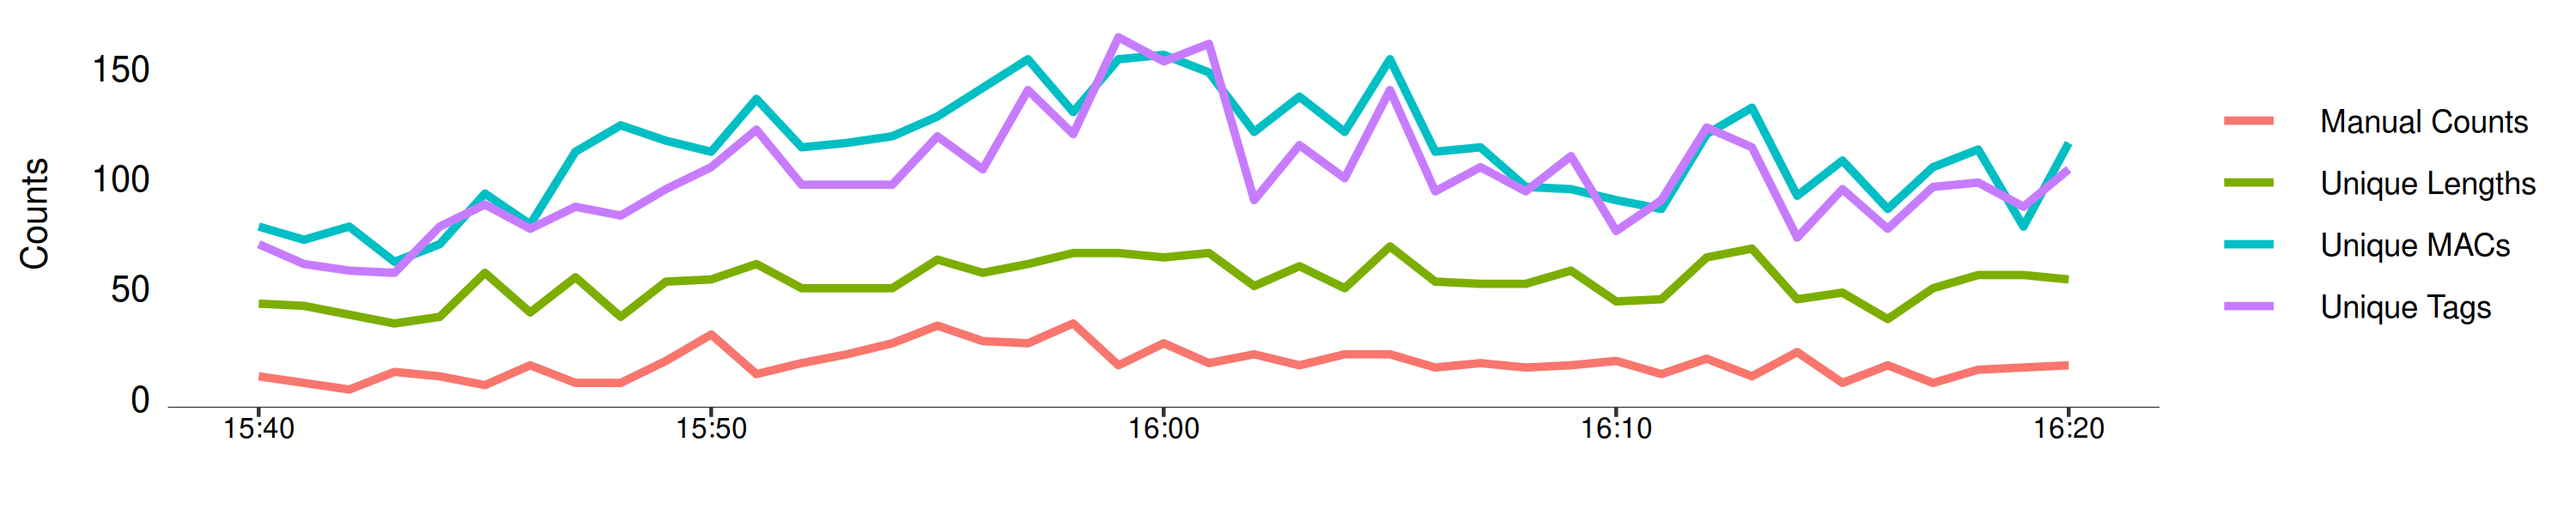
\includegraphics{images/ucl-comparison-before.png}
  \caption{Number of probe requests collected every minute on 15 October 2017}
  \label{figure:collection:ucl:before}
\end{figure*}

The second step was to see how much the sensor collected counts differ from the manual counts.
We aggregated the sensor counts for every minute in terms of the number of probe requests, unique MAC addresses and the unique frame lengths and compared them to the manual counts done for each minute.
The results are shown in Figure \ref{figure:collection:ucl:before}.
We can observe that the original Mean Average Percentage Error (MAPE) is around -----.
This was reduced to ----- and ----- when aggregated by MAC address and frame lengths but we see that it not accurate enough on its own.

\lipsum[1] Just by filtering to -70dBm reduces MAPE to \%.

\begin{figure*}
  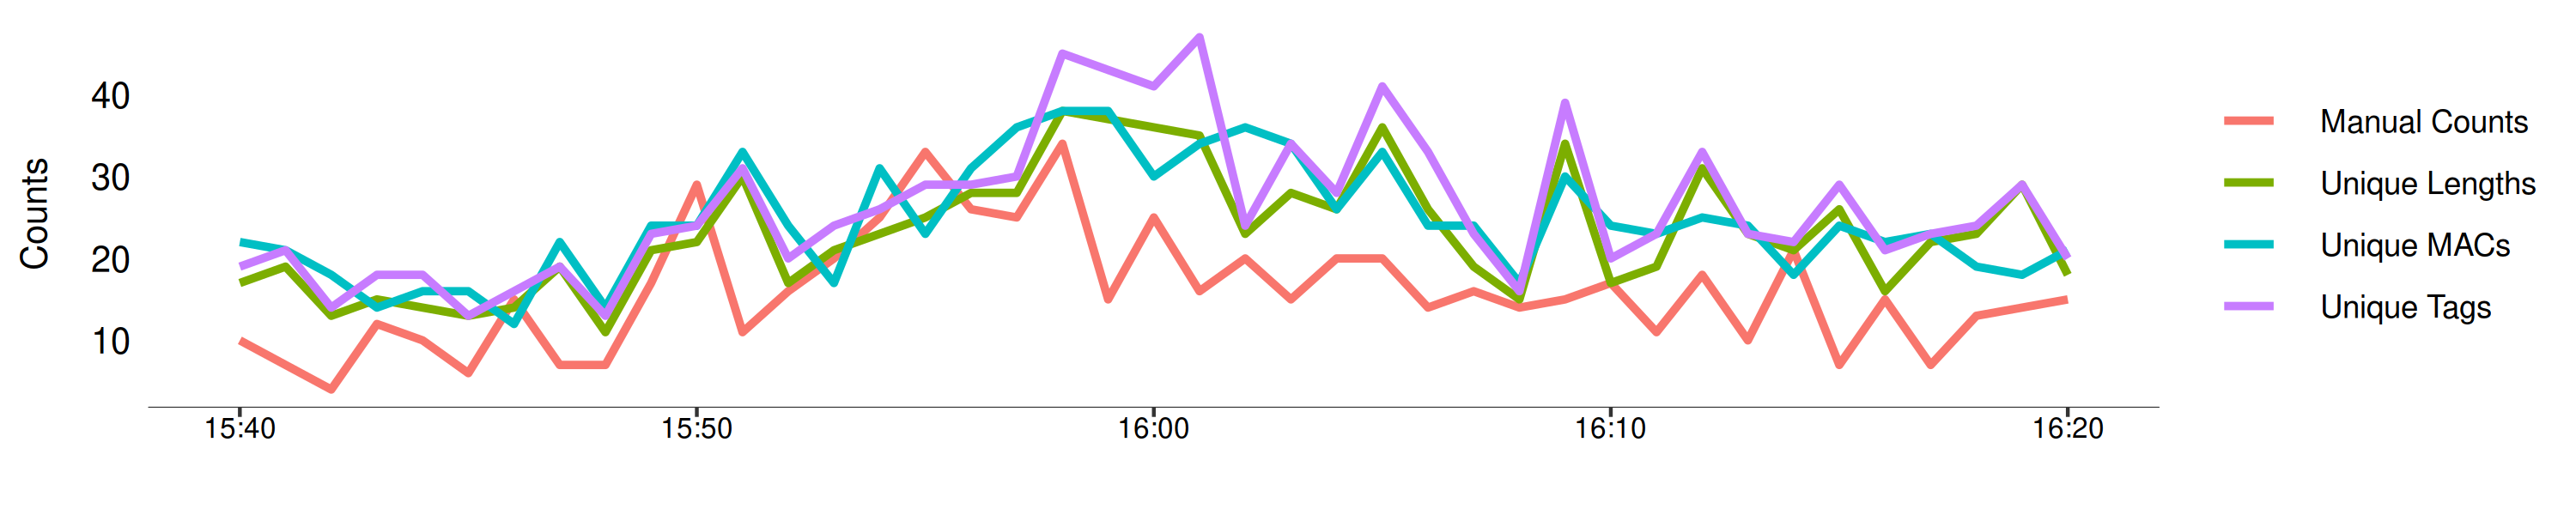
\includegraphics{images/ucl-comparison-after.png}
  \caption{Number of probe requests collected every minute on 15 October 2017}
  \label{figure:collection:ucl:config}
\end{figure*}

Major conclusion is that confirmation that Signal strength is still useful.
The signal number is just arbitrary. We need a way to calculate this.
fig \ref{} shows the distribution of signal along with breaks calculated by kmeans.
There is a break point. may be use some one dimensional breaks algorithm to find this dynamically.
Length information is not that useful in certain standardised manufacturers.
eg of randomised mac addresses and apple addresses.
This data set is ruined by the student bias, we need to have more real life data for actual analysis.
At larger scales the manual counting is not possible without errors need to make a better alternative.

\begin{figure}
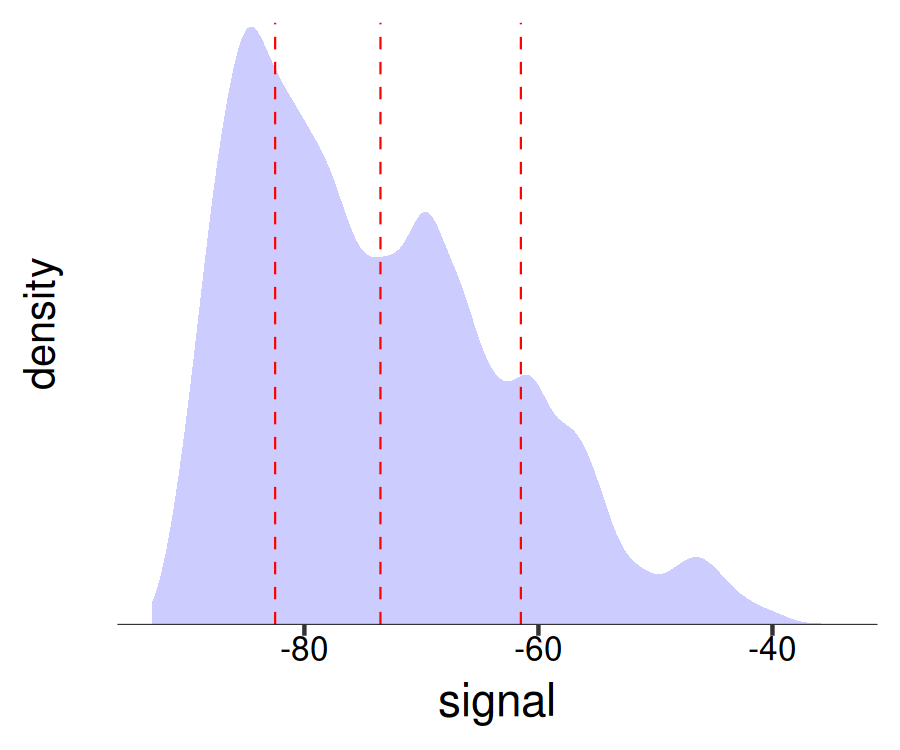
\includegraphics[trim={5 5 5 5},clip]{images/ucl-signal-dist.png}
  \caption{Number of probe requests collected every minute on 15 October 2017}
  \label{figure:collection:ucl:signal}
\end{figure}
\marginnote{\textit{} }

\lipsum[1]

%------------------------------------------------------------------------------%
\subsection{Oxford Street}
%------------------------------------------------------------------------------%

\begin{marginfigure}
  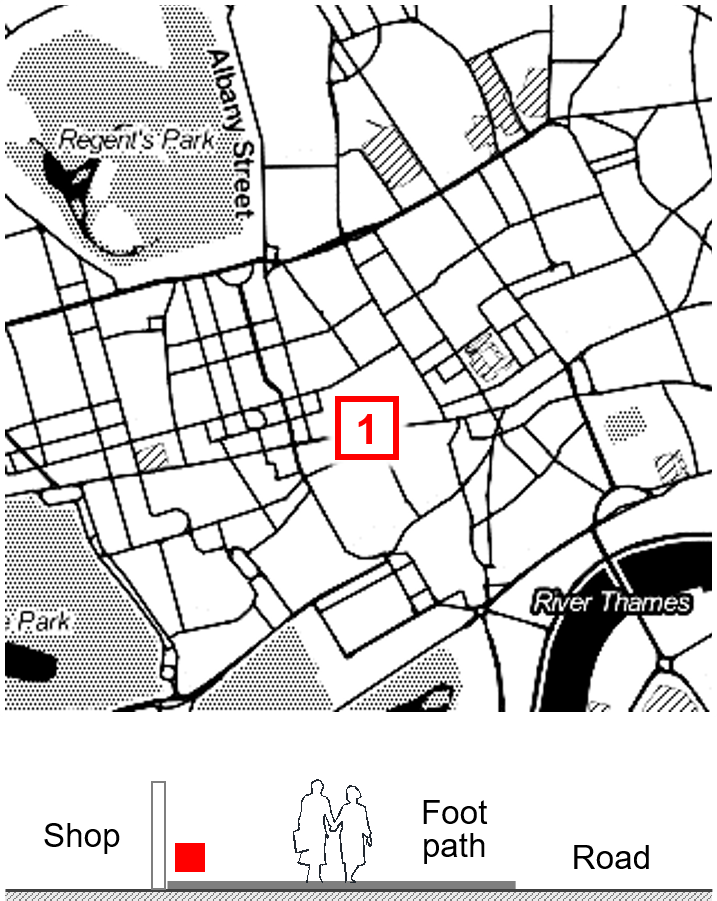
\includegraphics[trim={0 0 0 0},clip]{images/oxst-map.png}
  \caption{Number of probe requests collected every minute on 15 October 2017}
  \label{figure:collection:ucl:config}
\end{marginfigure}

From the learnings from the previous two experiments we need to devise a final `real world' experiment which collects high density data at a high street.
the Aim is to generate a dataset which can be used to test and validate signal strength based filtering and sequence number based clustering methodology against the scale and complexity of a busy, open public area such as a retail high street.
The location chosen was Oxford street, London - one of the busiest retail streets in the world.
The data was collected from 12:30 - 13:04 hrs on 20 December 2017 using the same methodology as above from a laptop in a backpack.
The surveyor positioned himself at the front of a store while carrying the backpack and counted people walking by the store on the pavement (3m wide approximately) using a mobile phone.
The sensor was kept as close to the store window as possible, and the manual count was done as a cordon count in front of the store.
The manual counting was done using a node-js base command line app running under Termux on an android phone.
The application is detailed in section \ref{appendix:manualcount} which counts the number of times a key has been pressed on the phone.
This has an additional advantage as the phone used is kept unconnected to any Wi-Fi and with the screen on for counting, emits probe requests at regular intervals.

\begin{marginfigure}
  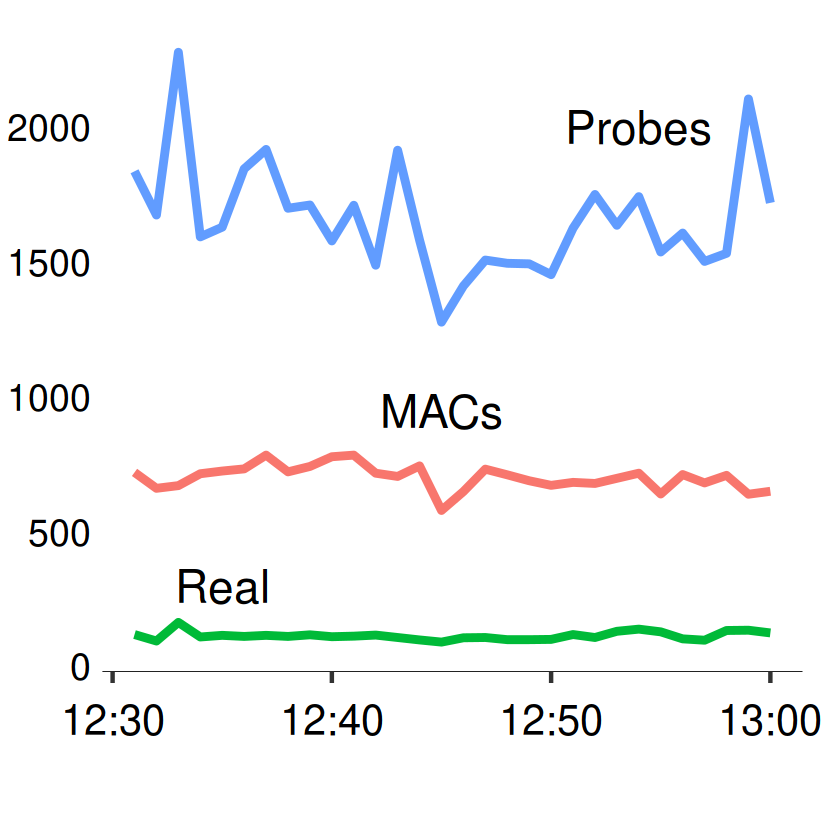
\includegraphics[trim={0 0 0 0},clip]{images/oxst-counts.png}
  \caption{Number of probe requests collected every minute on 15 October 2017}
  \label{figure:collection:ucl:config}
\end{marginfigure}

Moreover we know the phone to be of the vendor 'Google' and randomises the MAC address, giving us a good base line to compare our results to.
The Wi-Fi sensor captured approximately 60,000 probe requests during the half hour period; 3,722 people were manually recorded walking on the pavement during that time.
Initial exploration showed in Figure \ref{} that the data has large amount of noise and with \% of local mac addresses, it is free from high concentration of global mac addresses as we saw in the data from UCL corridors.
This dataset is extensively used in the development of the filtering and cleaning methods and which are discussed in detail on Section \ref{}

%------------------------------------------------------------------------------%
\subsection{Discussion}
%------------------------------------------------------------------------------%
Probe requests are source of easy to collect rich information.
We identified list of useful information we can get from them.
We collected data in three phases starting from small isolated study, more footfall and real world retail location.
The first experiment showed that MAC address is not enough. Local mac addressed can be publicly registered as well.
Signal strength is crucial.
The broader UCL experiment in UCL corridor showed that though length information looked useful, it fails with apple devices since they are very similar to each other and lack any information elements. 
This gave us a good idea of what to collect in a field study. 
We collected data at Oxford street as a dataset for to be used as a starting point for any methodology we develop further.

%==============================================================================%
